\documentclass[../MaxHughesThesis.tex]{subfiles}

\begin{document}
To obtain a measure of the Fierz term, the beta energy spectrum must be accurately described.
The description of the beta energy spectrum is written as a series of corrections multiplying the main phase space factor.  
Through out this chapter, $\hbar = c = 1$.

The beta energy spectrum shape can be broken up in three different factors. 
The three terms are written out as  %in equation \ref{eq:betaspectrum}

\begin{equation}
	\frac{dN}{dE} = PS(E) \times C(E) \times (1 + b_{GT}\frac{m_{e}}{E})
	\label{eq:betaspectrum}
\end{equation}
$PS(E)$ is the phase space of the electron, $C(E)$ are all the hadronic and electromagnetic corrections multiplied together, and $b_{GT}$ the Fierz term.
This chapter will describe all that goes into the determining the beta energy spectrum.

\section{Experimental Inputs to Describe the Beta Spectrum}
The corrections depend on several parameters of the decay. 
Some of them are just numbers, such as the atomic number of the daughter or mother nucleus or the mass number of the system.
However, there are two important parameters that extracted from experimental measurements and therefore have some uncertainty.
One is the $Q$-value of the decay, which is defined as %in equation \ref{eq:qval}.

\begin{equation}
	Q = m_{^{20}F} - (m_{^{20}Ne} + E_{level})
	\label{eq:qval}
\end{equation} 
where $m_{^{20}F}$ is the nuclear mass of $^{20}$F, $m_{^{20}Ne}$ is the nuclear mass of $^{20}$Ne, and $E_{level}$ is the energy of the 1.6 MeV nuclear state in $^{20}$Ne. 
The tabulated masses for these nuclei are the atomic masses, $M$, which differ from the nuclear masses by the electron mass and the binding energy of the electrons.
The electron masses are subtracted off, since the binding energy of the electrons is insignificant.
For $^{20}$F, $M_{20Ne} = 19.9924401762 (17)$ amu, $M_{20F} = 19.999981252 (31) $ amu \cite{Wan17} , and $E_{level} = 1.633674 (15)$ MeV  \cite{Til98} .

This mass difference is not quite the maximum electron energy. 
To get to the maximum electron energy, $E_{0}$, the energy of the recoiling nucleus has to be taken into account.
The formula is \cite{Hol74}%shown in equation \ref{eq:recoilqval}

\begin{equation}
	E_{0} = Q \left( \frac{1 + \frac{m_{e}^{2}}{2M_{ave} Q}}{1 + \frac{Q}{2M_{ave}}} \right)
	\label{eq:recoilqval}
\end{equation} 
with $m_{e}$ is the electron mass and $M_{ave}$ is the average nuclear mass. 

The other parameter is the charge radius of the daughter nucleus.
There are several ways to calculate the charge radius.
In this work, the charge radius was taken from the measured root mean square (RMS) charge radius and converted to the charge radius $R$.
It was assumed that the $^{20}$Ne nucleus was a sphere. 
From this, the radius was calculated using %equation \ref{eq:sphereeq}
\begin{equation}
	R = \sqrt{\frac{5}{3}}r_{rms}	
	\label{eq:sphereeq}
\end{equation}
where $r_{rms}$ is the root mean square charge radius, and $R$ the charge radius.
For this work, $r_{rms} = 3.0055 (21)$ fm \cite{Ang13}.

\section{Phase Space Factor}
The main part of the beta energy spectrum is the phase space factor.
It is %shown in equation \ref{eq:phase_space}

\begin{equation}
	\frac{dN}{dE} = C \times p_{e}W(W_{0} - W)^{2}
	\label{eq:phase_space}
\end{equation}
where $dN/dE$ is the spectrum of electrons emitted as a function of energy, $C$ is a constant, $p_{e}$ is the electron momentum, $W$ the total electron energy divided by $m_{e}$, and $W_{0}$ the maximum electron energy divided by $m_{e}$.
This is derived from the density of states of the particle when the neutrino degrees of freedom are integrated over.
The constant has factors that come from that integration.

\section{Variables of the Correction Factors}

For the rest of the discussion of the corrections to the energy spectrum, everything is given without units.
These corrections are largely electromagnetic in origin.
All of the energies are divided by the electron mass.
For this work, $m_{e} = 0.510998928$ MeV.
The other important variables are shown in table \ref{tab:vars}.

\begin{table}[!hbt]
	\centering
	\caption{Variables used in the corrections.}
		\begin{tabular}{lrr}
		Variable & Description & Equation or Value \\ \hline		
		$A$ & Mass number & 20 \\ 
		$Z$ & Atomic number of daughter & 10 \\
		$\alpha$ & Fine structure constant & 1/137.0359\\
		$R$ & Charge radius of daughter & 3.944 fm \cite{Ang13} \\
		$W$ & Total energy of the electron & $E/m_{e}$ \\
		$p$ & Electron momentum & $\sqrt{W^{2} - 1}$ \\
		$W_{0}$ & Maximum electron energy &  5.900864 (82) MeV \\ 
		$M_{ave}$ & Average nuclear mass &  18621.497033 (40) MeV  \\
		$\gamma = \sqrt{1 - (\alpha Z)^{2}} $ & $\gamma$ factor & 0.9973 
		\end{tabular}
	\label{tab:vars}
\end{table}



\section{Electromagnetic Corrections and Hardonic Corrections}
A graph of the various electromagnetic corrections is shown in figure \ref{fig:corrections}, along with the hadronic shape factor. 

\begin{figure}
    \centering
    \begin{minipage}{0.65\textwidth}
        \centerline{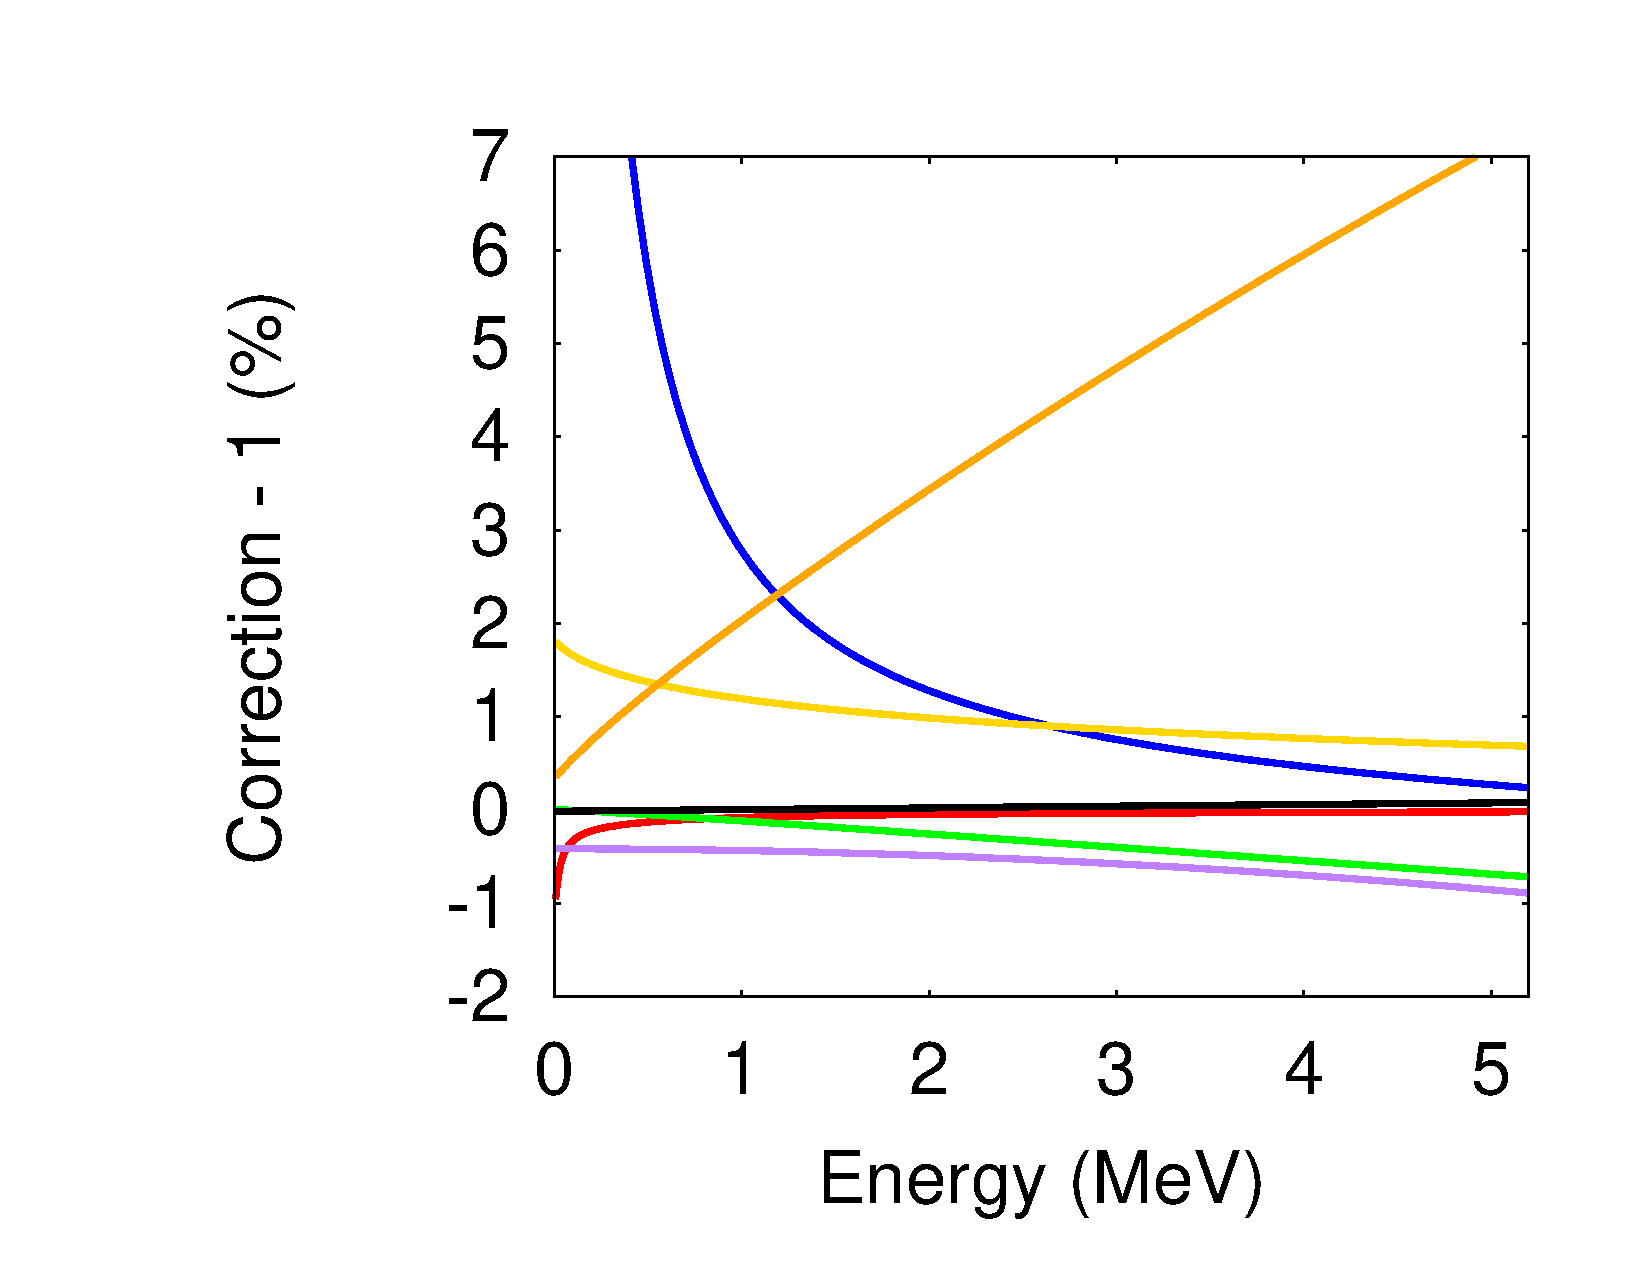
\includegraphics[width=0.9\textwidth]{Corrections_F20_ForCom_nokey.pdf}} % first figure itself
    \end{minipage}\hfill
    \begin{minipage}{0.35\textwidth}
        \centerline{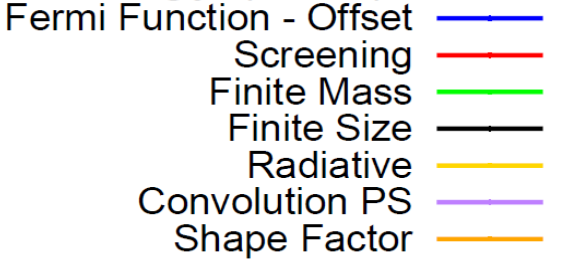
\includegraphics[width=0.9\textwidth]{Corrections_F20Key.png}}
    \end{minipage}
    \caption{Electromagnetic and hardonic corrections for $^{20}$F.
	     Plotted are the Fermi function \cite{Wil89}, the screening correction \cite{Buh84}, the finite mass correction \cite{WIL90}, the finite size correction \cite{WIL90}, the radiative correction \cite{Fay86}, the convolution of phase space correction \cite{WIL90}, and the hadronic shape factor \cite{Cal77}.}
    \label{fig:corrections}
\end{figure}

\subsection{Fermi Function}

In absolute value, the largest correction is the Fermi function.
This accounts for the interaction of the charge of the outgoing electron and the charge of the nucleus.
It is calculated by taking the Dirac equation wave functions and assuming the nucleus is a point charge of $Ze$.
The Dirac wave functions are taken down to a nuclear radius $R$.
This is since the wave functions diverge \cite{Wil89}.
The Fermi function is %printed in equation \ref{eq:fermifunc}
\begin{equation}
	F(Z,W) = 2\frac{\gamma + 1}{\Gamma(2\gamma +1)^{2}}(2pR)^{2(\gamma - 1)}e^{\frac{\pi\alpha ZW}{p}}\|\Gamma(\gamma + i\frac{\alpha ZW}{p})\|^{2}
	\label{eq:fermifunc}
\end{equation}
While this is the largest correction, it is the most understood one.
There is no change of shape due the uncertainty in $R$ because it alters as a factor the functional form of the Fermi function. 

\subsection{Radiative Correction}
The radiative correction is the next largest electromagnetic correction.
For this measurement, the correction is only needed to first order, which is on order $\alpha$.
The correction is a QED correction that stems from photons emitted from the beta particle.
This photon can be absorbed by the nucleus of the daughter, which makes it a virtual photon.
The photon can also be a real photon that propagates off to infinity.
The real photons are known as inner bremsstrahlung.

There are different descriptions of the radiative correction.  
The standard is by Sirlin \cite{Sir67} and is %shown in equation \ref{eq:sirlinrad}.

\begin{equation}
	\label{eq:sirlinrad}
	\begin{split}
	R(W,W_{0}) = & 1 + \frac{\alpha}{2\pi}[3\ln(M_{p}) - \frac{3}{4} + 4(\frac{\arctanh(\beta)}{\beta} - 1)\times(\frac{W_{0} - W}{3W} - \frac{3}{2} + \ln(2(W_{0} - W))) \\
	 & + \frac{4}{\beta}L \left(\frac{2\beta}{1 + \beta}\right) + \frac{\arctanh(\beta)}{\beta}\times(2\times(1 + \beta^{2}) + \frac{(W_{0} - W)^{2}}{6W^{2}} - 4 \arctanh(\beta))]
	\end{split}
\end{equation} 
with $\beta = \frac{p}{W}$, $M_{p}$ the proton mass divided by the electron mass, and $L(\frac{2\beta}{1+\beta})$ referring to the Spence function, which is \cite{Wil95} %as seen in equation \ref{eq:spence} \cite{Wil95}

\begin{equation}
	L(x) = \int_{0}^{x} \frac{\ln(1 - t)}{t}dt
	\label{eq:spence}
\end{equation}
The Sirlin formula assumes that the inner bremsstrahlung photons are not detected at all.
This is mostly true if the source of the beta decay is outside of a detector.
However, if the source is implanted inside of the detector, such as it is in this experiment, some of the inner bremsstrahlung is absorbed.

If all of the inner bremsstrahlung is absorbed, a different form of the first order radiative correction is needed.
There are many equivalent forms of this, but the one that was used for this experiment was by Fayans \cite{Fay86}.
The form of this radiative correction is %shown in equation \ref{eq:fayansrad}
\begin{equation}	
	\label{eq:fayansrad}
	\begin{split}
	R(W,W_{0}) = & 1 + \frac{\alpha}{\pi}[(\frac{2}{\beta}\ln \left( \frac{2\beta}{1+\beta} \right) + \frac{7}{8\beta} + \frac{3\beta}{8})\ln \left(\frac{1 + \beta}{1 - \beta} \right) \\
	& - 2\ln \left(\frac{4\beta^{2}}{1 - \beta^{2}}\right) + \frac{4}{\beta}L \left(\frac{2\beta}{1+\beta}\right) + \frac{23}{8} + \frac{3}{2}\ln(M_{p})]
	\end{split}
\end{equation}
The amount of inner bremsstrahlung absorbed depends obviously on the geometry.
Since the detector is small enough not to absorb all of the inner bremsstrahlung, a more careful treatment of the radiative correction is needed.

\subsubsection{Inner Bremsstrahlung}

To first order, the energy spectrum of the inner bremsstrahlung photons is independent of $Z$.
This is exactly like the two radiative corrections shown in equations \ref{eq:sirlinrad} and \ref{eq:fayansrad}. 
The spectrum is written as \cite{Kni36}%in equation {\ref{eq:KUB} \cite{Kni36}

\begin{equation}
	\Phi(k,W_{e}) = \frac{ \alpha p}{ \pi p_{e} k} [\frac{W_{e}^{2} + W^{2}}{W_{e}p}log(W + p) - 2]
	\label{eq:KUB}
\end{equation}
where $\Phi(k,W_{e})$ is the probability density of emitting a photon of energy $k$ from an electron of initial energy $W_{e}$.
This equation was derived using outgoing waves from the Dirac equation in polar coordinates.
This was calculated with the first order Born approximation.
This means that at low energies, equation \ref{eq:KUB} is inaccurate. 
That can be seen, as the equation diverges as $k$ goes to zero.
If more orders of the approximation are added, this divergence can be controlled.
These higher orders would correspond to emitting multiple photons.
Each of these orders would have a probability reduced by a factor of $\alpha$ compared to equation \ref{eq:KUB}.
The higher orders would be less significant, except at low energies, where the probability density diverges.
This would make the probability of emitting no photons finite.	 		
However, another possibility is to add a cutoff. 
As long as the cutoff is high enough to be in the region where the first order Born approximation is valid, but low enough not to cut out gamma rays that are not fully absorbed, equation \ref{eq:KUB} is valid.
The cutoff used was 50 keV.
This cutoff was checked using Monte Carlo simulation, and is within the region where the detector and the source geometry absorbs all gamma rays.

To quantify the effect of the inner bremsstrahlung, a GEANT4 simulation was used.
Electrons were generated using the phase space and the radiative correction in equation \ref{eq:fayansrad}.
Then, for each electron, equation \ref{eq:KUB} was sampled and a photon generated.
No other physics process was looked at in this simulation.
The ratio consisting of the energy absorbed over the initial energy was the output of the simulation.
That ratio is the effective efficiency of absorbing the inner bremsstrahlung photons.
Multiplying that ratio by equation \ref{eq:fayansrad} gives the effective radiative correction.
The comparison of all three radiative corrections is shown in figure \ref{fig:rad}.

\begin{figure}[!htb]
	\centerline{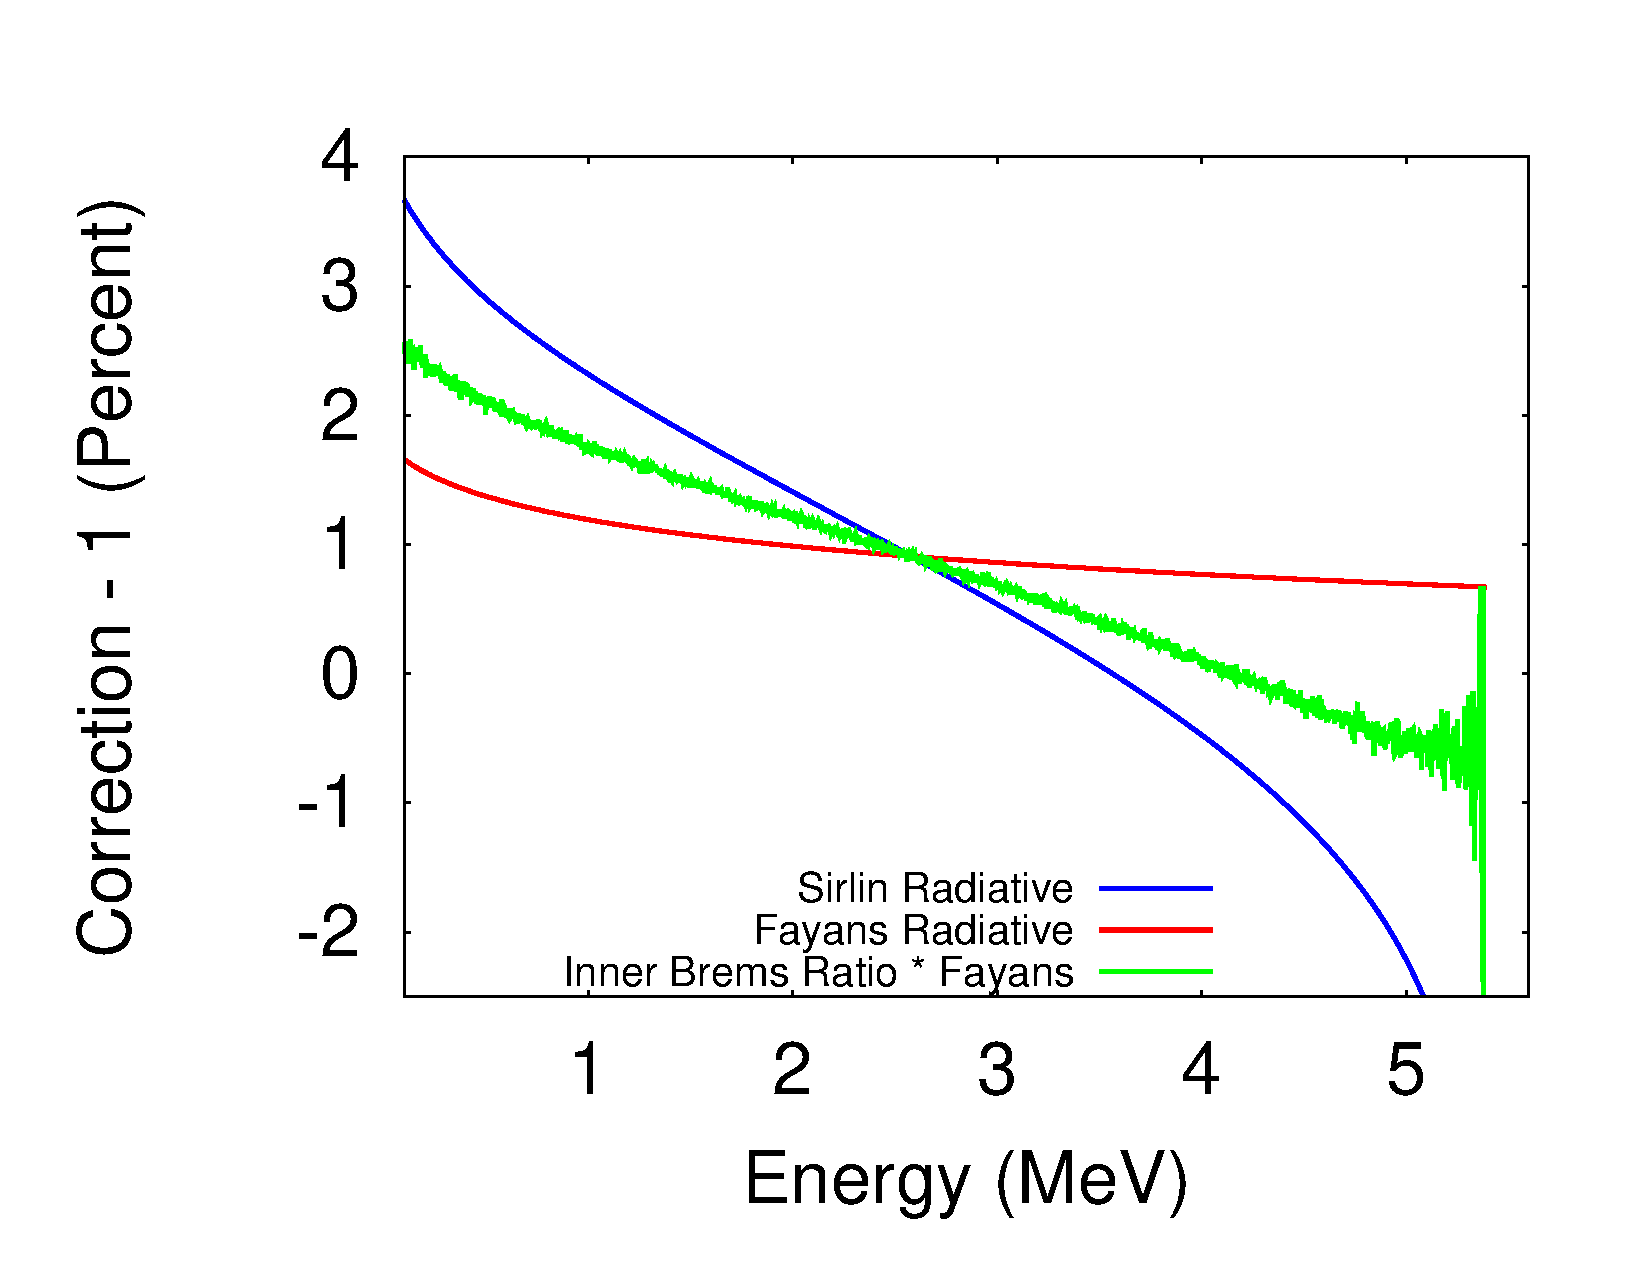
\includegraphics[width=0.61\textwidth]{RadCorrections_20F.pdf}}
	\caption{Comparison of three different radiative corrections.
		 The green line depends strongly on the detector geometry.
		 }
	\label{fig:rad}
\end{figure}
The effect of the inner bremsstrahlung for a finite detector is to put the radiative correction halfway between the Sirlin and the Fayans formulas.

\subsection{Screening}
The screening correction is the next largest electromagnetic correction.
This is a correction to the Fermi function.
It corresponds to the screening of the nuclear charge due to the electron cloud of the atom.
The strongest effect of the screening correction is at low electron energies and for large atomic numbers.

\subsubsection{Potentials Used in Screening Derivation}
To calculate this correction, the Coulomb potential used to calculate the Fermi function is replaced with a Hulth\'en potential.
This potential is %shown in equation \ref{eq:hulth}

\begin{equation}
	V(r) = -\frac{\alpha Z \beta}{e^{\beta r} - 1}
	\label{eq:hulth}
\end{equation}
where $r$ is the distance away from the center and $\beta$ is a parameter characterizing the diffuseness of the electron cloud.
The ratio of this new Fermi function to the old Fermi function is the screening correction which multiplies the phase space. 

The screening correction is negligible except near the origin, while near the origin, equation \ref{eq:hulth} behaves as %equation \ref{eq:hulthorg}

\begin{equation}
	V(r) = -\frac{\alpha Z}{r} + \frac{1}{2}\alpha Z \beta
	\label{eq:hulthorg}
\end{equation}
and $\beta$ is given by \cite{Buh84} %equation \ref{eq:screenbeta} \cite{Buh84}. 
	
\begin{equation}
	\beta = 2C(Z)\alpha Z^{1/3} m_{e}
	\label{eq:screenbeta}
\end{equation}
Here, the $Z$ is number the electrons of the daughter atom because the assumption is that beta decay is occurring from neutral atoms.
The only unknown is $C(Z)$.

To find the value of $C(Z)$, a comparison is needed. 
In another method of describing screening, the potential is described as a series of exponentials.
This is written as \cite{Bya56} %shown in \ref{eq:hart} \cite{Bya56}.

\begin{equation}
	V(r) = -\frac{\alpha Z}{r}\sum_{n}c_{n}e^{-b_{n} x}
	\label{eq:hart}
\end{equation}
where $b_{n}$ and $c_{n}$ are constants.
The sum of all the $c_{n}$ adds up to one.
The value of $x$ is \cite{Bya56} %shown in equation \ref{eq:screeningx} \cite{Bya56}

\begin{equation}
	x = 1.13 \alpha Z^{1/3} r m_{e}
	\label{eq:screeningx}
\end{equation}
When equation \ref{eq:hart} is expanded near the origin and $x$ is written explicitly, the result is %equation \ref{eq:hartorg}

\begin{equation}
	V(r) = - \frac{\alpha Z}{r} + \frac{1}{2} \alpha Z \times 2 (1.13 \sum_{n} b_{n} c_{n}) \alpha Z^{1/3} m_{e} 
	\label{eq:hartorg}
\end{equation}
By comparing equations \ref{eq:hulthorg} and \ref{eq:screenbeta} with \ref{eq:hartorg}, the result obtained is %in equation \ref{eq:betaanswer} are obtained.

\begin{equation}
	C(Z) = 1.13 \sum_{n} c_{n} b_{n}
	\label{eq:betaanswer}
\end{equation} 
There is only one term in $^{20}$F. 
The parameters in equation \ref{eq:betaanswer} are $c_{1} = 1$ and $b_{1} = 0.907$ \cite{Bya56}.

\subsubsection{Screening Correction Formula}
From equation \ref{eq:betaanswer}, the factor $C(Z)$ in equation \ref{eq:screenbeta} is evaluated $0.907 \times 1.13 = 1.02491$.
Equation \ref{eq:hulthorg} can then be used to calculate the screening correction.
The result is \cite{Buh84} %shown in equation \ref{eq:screeningQ} \cite{Buh84}.

\begin{equation}
	Q(Z,W) = X(\frac{W'}{W}) \left|\frac{\Gamma(\gamma + i y')}{\Gamma(\gamma+ i y)}\right|^{2} \left|\frac{\Gamma(\gamma + 2 i \frac{p'}{\beta})}{\Gamma(\gamma + 2 i \frac{p}{\beta})}\right|^{2}e^{-\pi y}(\frac{2p}{\beta})^{2(1 - \gamma)}
	\label{eq:screeningQ}
\end{equation}
with $y = \frac{\alpha Z W}{p}$, $y' = \frac{\alpha Z W'}{p'}$,$ \gamma$ is in table \ref{tab:vars}, $W' = W - \frac{1}{2}\alpha Z \beta$, and $p' = \frac{1}{2}p + \frac{1}{2}\sqrt{p^{2} - 2 \alpha Z W' \beta}$.

$X(\frac{W'}{W})$ is %in equation \ref{eq:screeningX}
\begin{equation}
	X = \frac{1 + \frac{W' + \gamma m_{e}}{8 W'} (\frac{\beta}{p})^{2} + \frac{1}{2}\gamma^{2}[1 + (1 - \frac{\alpha Z \beta}{(W + m_{e})})^{1/2}]^{-2} [\frac{W - m_{e}}{W'}] (\frac{\beta}{p})^{2}[1 - \frac{1 - \gamma}{8\gamma}(\frac{\beta}{p})^{2}]}{(1 + \frac{\beta}{4p}^{2})}
	\label{eq:screeningX}
\end{equation}
The factor $X$ in equation \ref{eq:screeningX} is very close to 1.
This correction matters mostly at low energy, and is very flat above 100 keV.

\subsection{Finite Mass Correction}
The finite mass correction accounts for the recoil motion of the $^{20}$Ne nucleus.
The form of finite mass corrections is given as \cite{WIL90} %in equation \ref{eq:finitemass} \cite{WIL90}

\begin{equation}
	R(W,W_{0},m_{^{20}Ne}) = 1 + r_{0} + \frac{r_{1}}{W} + r_{2}W + r_{3}W^{2}
	\label{eq:finitemass}
\end{equation}
The forms of the $r_{i}$ depend on if the decay is a vector decay or an axial decay. 
This is due to angular momentum conservation.
Since $^{20}$F is an axial decay, the finite mass correction coefficients are %shown in equations \ref{eq:finitemassrs} 

\begin{equation}
	\label{eq:finitemassrs}
	\begin{split}
	r_{0} & = -\frac{2W_{0}}{m_{^{20}Ne}} - \frac{W_{0}^{2}}{6(m_{^{20}Ne})^{2}} - \frac{77}{18(m_{ ^{20}Ne})^{2}} \\
	r_{1} & = -\frac{2}{3m_{^{20}Ne}} + \frac{7W_{0}}{9(m_{^{20}Ne})^{2}} \\
	r_{2} & = \frac{10}{3m_{^{20}Ne}} - \frac{28W_{0}}{9(m_{^{20}Ne})^{2}} \\
	r_{3} & = \frac{88}{9m_{^{20}Ne}}
	\end{split}
\end{equation}
This correction is different from the hadronic shape factor described later. 

\subsection{Finite Size Correction}
The finite size correction originates from treating the nucleus as a uniformly charged sphere instead of a point particle.
This sphere has a radius of $R$, as shown in equation \ref{eq:sphereeq}.
The form of the finite size correction is \cite{WIL90} %shown in equation \ref{eq:finitesize} \cite{WIL90}

\begin{equation}
	\label{eq:finitesize}
	\begin{split}
	L_{0}(Z,W) = 1 + \frac{13(\alpha Z)^{2}}{60} - \alpha Z W R \frac{41 - 26\gamma}{15(2\gamma - 1)} - \alpha Z R \gamma \frac{17 - 2\gamma}{30W(2\gamma - 1)}  \\
	+ a_{-1} \frac{R}{W} + \sum_{n=0}^{5} a_{n} (W R)^{n} + 0.41(R - 0.0164)(a Z)^{4.5}
	\end{split}
\end{equation}
Where the $a_{n}$ coefficients are parameterized by %equation \ref{eq:A}
\begin{equation}
	a_{n} = \sum_{x = 1}^{6} b_{x}^{n} (\alpha Z)^{x}
	\label{eq:A}
\end{equation}
The $b_{x}$ coefficients are numbers shown in table \ref{tab:bcoef}.

\begin{table}[!hbt]
	\centering
	\caption{Coefficients for finite mass correction.}
		\begin{tabular}{lrrrrrr}
		         & $b^{n}_{1}$ & $b^{n}_{2}$ & $b^{n}_{3}$ & $b^{n}_{4}$ & $b^{n}_{5}$ & $b^{n}_{6}$ \\ \hline
		$a_{-1}$ & 0.115 & -1.8123 & 8.2498 & -11.223 & -14.854 & 32.086 \\
		$a_{0}$  & -0.00062 & 0.007165 & 0.01841 & -0.053736 & 1.12691 & -1.5467 \\
		$a_{1}$  & 0.02482 & -0.05975 & 4.84199 & -15.3374 & 23.9774 & -12.6534 \\
		$a_{2}$  & -0.14038 & 3.64953 & -38.8143 & 172.1368 & -346.708 & 288.7873 \\
		$a_{3}$  & 0.008152 & -1.15664 & 49.9663 & -273.711 & 657.6292 & -603.7033 \\
		$a_{4}$  & 1.2145 & -23.9931 & 149.9718 & -471.2985 & 662.1909 & -305.6804 \\
		$a_{5}$  & -1.5632 & 33.4192 & -255.1333 & 938.5297 & -1641.2845 & 1095.358 
		\end{tabular}
	\label{tab:bcoef}
\end{table}

\subsection{Convolution of Lepton and Nucleon Wavefunctions}

This is the last of the relevant electromagnetic corrections.
In figure \ref{fig:corrections}, the name given is, ``convolution PS.''
This correction $C(Z,W)$ accounts for the interaction of the lepton and nucleon wavefunctions. 
The radial part of the nucleon wavefunctions is  modeled as a rectangle with width $R$.
Much like the finite size and mass corrections, this correction depends on the type of $\beta$ decay.
Since the decay of interest is an axial vector decay, the form of this correction is %shown in equation \ref{eq:nucandlepconv}
\begin{equation}
	C(Z,W) = 1 + C_{0} + C_{1} W + C_{2} W^{2}
	\label{eq:nucandlepconv}
\end{equation}
where the $C_{i}$ coefficients are defined as \cite{WIL90} %in equation \ref{eq:csconvocorrection} \cite{WIL90} 

\begin{equation}
	\label{eq:csconvocorrection}
	\begin{split}
	C_{0} & = -\frac{-233(\alpha Z)^{2}}{630} - \frac{(W_{0} R)^{2}}{5} + \frac{2 \alpha Z R W_{0}}{35} \\
	C_{1} & = -\frac{21 \alpha Z R}{35} + \frac{4 W_{0} R^{2}}{9} \\
	C_{2} & = -\frac{4 R^{2}}{9}
	\end{split}
\end{equation}
This correction depends on both the maximum energy of the outgoing electron and the charge radius.
The contribution from this correction to the shape is minimal. 

\subsection{Hadronic Corrections}

Nuclear form factors are one of the largest corrections to the beta spectrum.
There are four relevant form factors that come together into a correction called here the nuclear shape factor.
The form factors are listed in table \ref{tab:formfact} \cite{Cal77}.
The shape factor is written as 
\begin{equation}
	\label{eq:shapefactor}
	S(E) = 1 + c_{0} + c_{1} + \frac{c_{-1}}{E} + c_{2}E^{2}	
\end{equation}
where the terms depend on the form factors and nuclear decay variables.
\begin{table}[!hbt]
	\centering
	\caption{Nuclear form factors.}
		\begin{tabular}{lrr}
		Form Factor & Name & Value \\ \hline
		$c_{1h}$ & Gamow-Teller matrix element & 0.253  \cite{Min11}\\
		$c_{2h}$ & Second forbidden matrix element & 0.755 fm$^{2}$ \cite{Cal77} \\
		$b_{WM}$ & Weak magnetism & 43.4  \cite{Min11} \\
		$d$ & Induced tensor term & 40.5  \cite{Min11}
		\end{tabular}
	\label{tab:formfact}
\end{table}
The dependence of the coefficients $c_{i}$ is given by\cite{Cal77}

\begin{equation}
	\label{eq:sfcs}
	\begin{split}
	c_{0} & = -\frac{2 E_{0}}{M_{ave}}(1 + \frac{d}{c_{1h}} + \frac{b_{WM}}{c_{1h}})  + \frac{2 c_{2h}}{9 c_{2h}} 11 m_{e}^{2} \\
	c_{-1} & = -\frac{m_{e}^{2}}{3M_{ave}} (2 + \frac{2b_{WM}}{c_{1h}} + \frac{d}{c_{1h}})  - \frac{2 c_{2h}}{9 c_{1h}} 2 m_{e}^{2} E_{0}\\
	c_{1} & =  \frac{2}{3M_{ave}} (5 + \frac{b_{WM}}{c_{1h}}) + \frac{2 c_{2h}}{9 c_{1h}} 20 E_{0} \\
	c_{2} & = -\frac{40 c_{2h}}{9 c_{1h}} 
	\end{split}
\end{equation}
Three of the form factors, $b_{WM}$, $d$ and $c_{1h}$ are extracted from experimental data. 
$c_{2h}$ is calculated from nuclear theory. 
The extraction of $c_{1h}$ depends on the $ft$ value and is \cite{Min11}

\begin{equation}
	c_{1h}^{2} = \frac{2 ft_{0}}{ft_{20}}
	\label{eq:c1eq}
\end{equation}
where $ft_{0}$ is the $ft$ value of the Fermi super-allowed $\beta$ decays, and $ft_{20}$ the average of the $ft$ values of the decays of $^{20}$F and $^{20}$Ne.
This gives a value of $0.254 \pm 0.004$ \cite{Min11}.
The weak magnetism, $b_{WM}$, is of special theoretical interest. 

\subsubsection{The Weak Magnetism}
The form factor having the largest effect is the weak magnetism form factor. 
It can be calculated from the $M1$ analog gamma-ray decay strength.
This decay strength is from the 10.275 MeV analog state to the 1.634 MeV first excited state in $^{20}$Ne.
This is a $2^{+}$ to $2^{+}$ angular momentum transition, and a $1$ to $0$ isospin transition.
The decay strength, $\Gamma_{M1}$, can be used to extract $b_{WM}$.
This extraction is 

\begin{equation}
	b_{WM} = \sqrt{\frac{6\Gamma_{M1}M^{2}}{\alpha E_{\gamma}^{3}}}
	\label{eq:bwmcal}
\end{equation}
where $M$ is the nuclear mass and $E_{\gamma}$ the energy of the gamma ray.
This gives a value of $43.4 \pm$ 1.2 \cite{Min11}.

Getting a measurement of this value is of interest for two reasons.
One, it tests the Conserved Vector Current (CVC) hypothesis.
This hypothesis states that the weak interaction possesses a universal strength and a universal $V-A$ form \cite{Man58}.
In decays involving a $T = 1$ multiplet, the form of the calculation is equation \ref{eq:bwmcal}. 
This is the largest of the nuclear corrections, and can be determined from experimental data, which has a much smaller uncertainty than any theory calculations.
The second reason is more experimental.
It gives a parameter with which to benchmark the measuring techniques and the analysis.
If the analysis produces the expected value of $b_{WM}$, the same procedure should give a reliable value for $b_{GT}$.

\subsubsection{The Induced Tensor Form Factor}

From equation \ref{eq:sfcs}, the induced tensor form factor $d$ contributes to the corrections much in the same way as the Fierz term.
This form factor was measured by combining two data sets \cite{Min11}.
Both the decay of $^{20}$F and $^{20}$Ne were used to measure $d$.
One data set was the alignment of out-going electrons.
The alignment is a higher order polarization.
To describe the alignment, the nuclear form factors are needed.  
The measured alignments of both $^{20}$F and $^{20}$Ne were added to eliminate the form factors that changed sign between the two nuclei.
To eliminate the remaining form factors, an existing gamma-beta angular correlation measurement of both nuclei was added. 
That data set was used to eliminate the remaining form factors other than $d$.
This gave a value of $d/Ac_{1h} = 8.00 \pm 0.73$.
Using $A = 20$ and $c_{1h} = 0.253$, this gives $d = 40.5 \pm 3.7$. 

\section{Summary}

\begin{figure}[!htb]
	\centerline{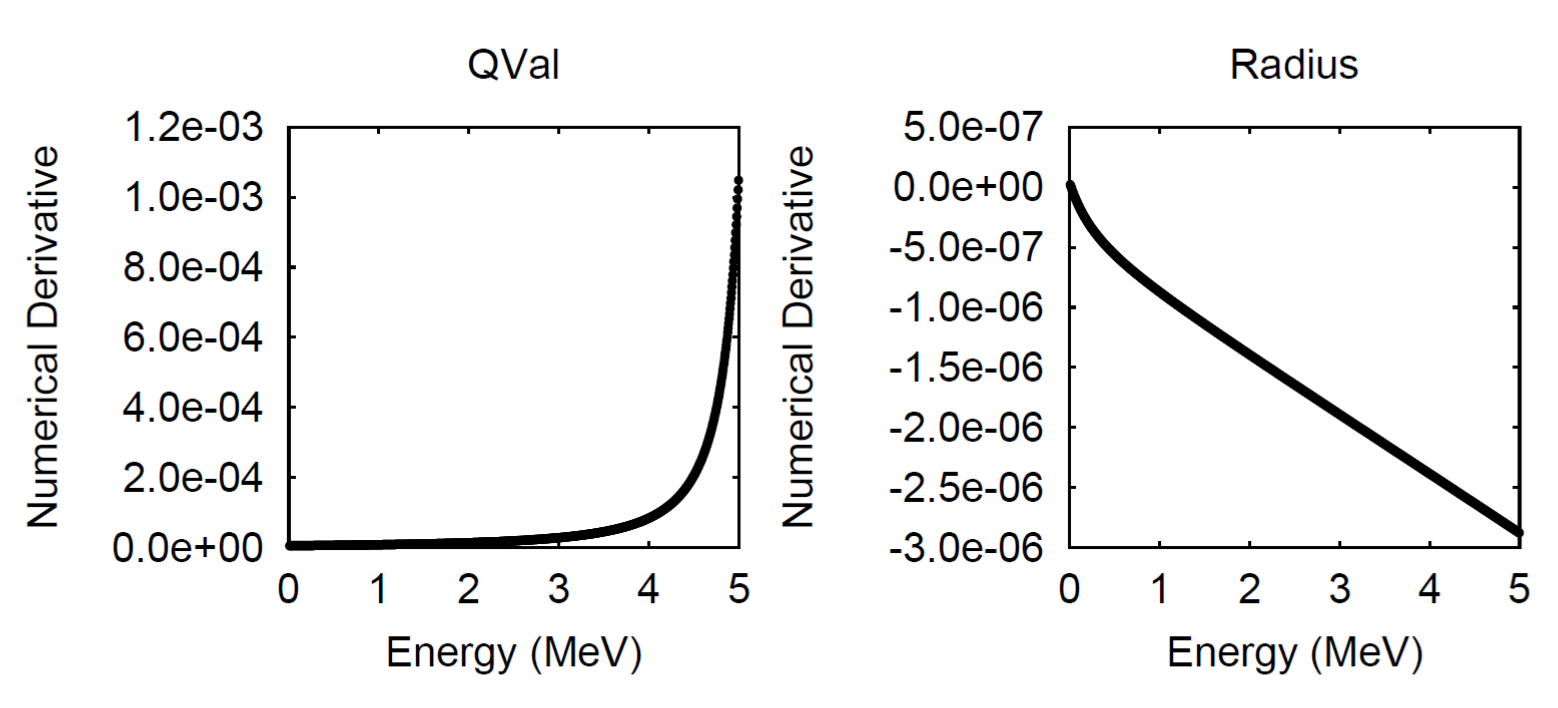
\includegraphics[width=0.75\textwidth]{DerivPlot_NoWeight.png}}
	\caption{The numerical derivative of the ratios in 1/MeV.
		 This is to check how sensitive the shape of the theoretical spectrum is to the uncertainty of the parameters extracted from experiment. 
		 These derivatives are order of an magnitude smaller than the 10$^{-2}$/MeV of the $c_{1}$ of the shape factor.}
	\label{fig:theoryuncer}
\end{figure}

Before the theoretical corrections were fed into a Monte Carlo simulation, the uncertainties from the experimentally determined quantities $R$ and $Q$ was checked.
The corrections and phase space were calculated with the central value of both parameters.
Then, two more spectra were calculated.
One was calculated with $R + eR$ instead of $R$, and the other was calculated with $Q + eQ$ instead of $Q$.
Here, $eR$ is the uncertainty of $R$ and $eQ$ the uncertainty of $Q$.
Two ratios were taken, which were $[PS(E,Q)C(E,Q,R+eR)]/[PS(E,Q)C(E,Q,R)]$ and $[PS(E,Q+eQ)C(E,R,Q+eQ)]/[PS(E,Q)C(E,Q,R)]$.
These results are shown in figure \ref{fig:theoryuncer}, where it is seen the change of shape induced is small.
The largest value of the numerical derivative is at the end point of the ratio of  $Q$. 
Even there it the ratio is smaller than the terms of the shape factor.
These results were further verified by generating a spectrum with a $b_{WM}$ and a $b_{GT}$.
This spectrum was fit with an additional generated spectrum with $R$ or $Q$ adjusted by one unit of uncertainty.
The change in the fit parameter was found to be smaller than the expected statistical uncertainty.

With all these corrections, the experiment can be described to the required precision.
\end{document}
